\documentclass[12pt, a4paper]{article}
\usepackage[utf8]{inputenc}

\usepackage{graphicx}

\usepackage{geometry}

\usepackage{multicol}
\usepackage{listings}


\usepackage{amsmath}
\usepackage{amsfonts}
\usepackage{amssymb}

\geometry{margin=0.6in}


\setlength{\parindent}{0em}
\setlength{\parskip}{1em}

\title{Analisi 1}


\begin{document}
\section{prime lezioni}
insiemi e logica elementare

numeri reali e naturali

\section{maggioranti, minoranti, sup e inf}

\textbf{Def}\\ Sia $A\in\mathbb{R}$ non vuoto.\\ $A$ è \textbf{limitato superiormente} se esiste $M\in\mathbb{R}$
tale che $x\leq M$ $\forall x\in A$. $M$ viene definito come \textbf{Maggiorante} di $A$. Se $M$ di $A$ appartiene
ad $A$ si dice \textbf{massimo} di $A$, e viene denotato come $max(A)$

$A$ è \textbf{limitato inferiormente} se esiste $m\in\mathbb{R}$ tale che $x\geq M$ $\forall x\in A$. $m$ viene
definito come \textbf{minorante} di $A$. Se $m$ di $A$ appartiene ad $A$ si dice \textbf{minimo} di $A$, e viene
denotato come $min(A)$

$A$ si dice \textbf{limitato} se è limitato sia inferiormente che superiormente

\textbf{Def}\\ Siano $A,B\in\mathbb{R}$ non vuoti
\begin{itemize}
    \item $-A \doteq \{-x \mid x\in A\}$
    \item $A+B \doteq \{x+y\mid x\in A,\ y\in B\}$
    \item $A-B \doteq \{x-y\mid x\in A,\ y\in B\}$
\end{itemize}
Se $x\in\mathbb{R}$
\begin{itemize}
    \item $x+A\doteq\{x+y\mid y\in A\}$
\end{itemize}

non importante, skippo

\section{lezioni skippate}
Caratterizzazione sup, inf, classi contigue, densità dei razionali

\section{Radici, esponenziali reali, funzioni inverse, logaritmi, trigonometriche}

\textbf{Prop - Radici n-esima}\\
per ogni numero nullo positivo $a$ e per ogni $n\in\mathbb{N}$ esiste un unico numero reale $b$ tale
che $b^{n}=a$. Tale reale positivo è la radice n-esima e si indica con i simboli:
\begin{center}
    $\sqrt[n]{a}\quad\doteq\quad a^{\frac{1}{n}} $
\end{center}

Sia $r\in\mathbb{Q},  r=\frac{p}{q},  p\in\mathbb{Z}  q\in\mathbb{N}$. Allora se $a>0$:
\begin{center}
    $a^{r}\doteq a^{\frac{p}{q}}\doteq \sqrt[q]{a^{p}} \qquad r\geq 0$

    $a^{r}\doteq a^{\frac{p}{q}}\doteq \frac{1}{\sqrt[q]{a^{-p}}} \qquad r<0$
\end{center}

La radice possiede le stesse proprietà della potenza intera

Se $0<a<1$, allora posto $b=\frac{1}{a}$ e definisco:
\begin{center}
    $a^{x}=\frac{1}{b^{x}}$
\end{center}

\textbf{Operazioni tra funzioni}\\$f,g$
    \begin{itemize}
        \item Somma: $(f+g)(x)\doteq f(x)+g(x)\qquad x\in dom(f)\cap dom(g)\neq \emptyset$
        \item Prodotto: $(f\times g)(x)\doteq f(x)\times g(x)\qquad x\in dom(f)\cap dom(g)\neq \emptyset$
        \item Rapporto: $(\frac{f}{g})(x)\doteq \frac{f(x)}{g(x)}\qquad x\in dom(f)\cap dom(g)\neq \emptyset
                  , g(x)\neq 0$
        \item Composizione: $(f\circ g)(x)\doteq f(g(x))\qquad \forall x\in A$
        \item Restrizione: $f:A\rightarrow\mathbb{R}\quad A\subseteq\mathbb{R},  A\neq\emptyset$. Se prendo
              $B\subseteq A$ allora la resitrzione $AB$ di $f$ è: $f\upharpoonright_{B}:  B\rightarrow\mathbb{R}$
    \end{itemize}

    \textbf{Def - funzioni limitate}\\ Sia $f:A\rightarrow\mathbb{R},  A\subseteq\mathbb{R}  A\neq\emptyset$,
    diremo che $f$ è \textbf{limitata superiormente} se $f(A)\subseteq\mathbb{R}$ è limitata superiormente,
    cioé esiste $M\in\mathbb{R}$ tale che $f(x)\leq M\quad \forall x\in A$. Analogamente diremo che $f$ è
    \textbf{limitata inferiormente} se $f(A)\subseteq\mathbb{R}$ è limitata inferiormente, cioé esiste
$m\in\mathbb{R}$ tale che $f(x)\geq m\quad \forall x\in A$.\\La funzione $f$ sarà \textbf{limitata} se
    è limitata inferiormente e superiormente.

    Quindi se $f(A)$ è limitata superiormente allora esiste il suo estremo superiore $sup(f(A))$, ovvero
$sup(f)\doteq sup(f(A))$. Lo stesso vale per l'opposto ($inf(f)\doteq sup(f(A))$).\\ Se $x_{0}\in dom(A)$
    e $f(x_{0})=sup(f)$ si dice che $f$ ammette \textbf{massimo assoluto}. Nel caso dell'estremo inferiore,
    diremo che $f$ ammette \textbf{minimo assoluto}

    \textbf{Def - funzioni monotone}\\Sia $f:A\rightarrow\mathbb{R},  A\subseteq\mathbb{R}  A\neq\emptyset$.
    Allora $f$ è detta:
    \begin{itemize}
        \item Crescente: per ogni coppia $x_{1},x_{2}\in A$, se $x_{1}<x_{2}\Rightarrow f(x_{1})\leq f(x{_2})$
        \item Strettamente crescente: per ogni coppia $x_{1},x_{2}\in A$, se $x_{1}<x_{2}\Rightarrow f(x_{1})<f(x{_2})$
        \item Decrescente: per ogni coppia $x_{1},x_{2}\in A$, se $x_{1}<x_{2}\Rightarrow f(x_{1})\geq f(x{_2})$
        \item Strettamente Decrescente: per ogni coppia $x_{1},x_{2}\in A$, se $x_{1}<x_{2}\Rightarrow f(x_{1})>f(x{_2})$
    \end{itemize}
    Le funzioni crescenti e decrescenti vengono definite monotone, mentre quelle strettamente crescenti o decrescenti
    sono strettamente monotone

    \textbf{Prop}\\Ogni funzione strettamente monotona è iniettiva

    Osservazioni:\\se $f$ è iniettiva, non per forza è strettamente monotona, ma vale la negazione: se una funzione
    non è iniettiva, allora sicuramente non è strettamente monotona.

    \textbf{Def - Funzioni inverse}\\Sia $A\subseteq\mathbb{R}$ non vuoto e $f:A\rightarrow B$. Se $f$ è biunivoca
    (iniettiva e suriettiva) allora $f$ è \textbf{invertibile} e si chiama funzione inversa di $f$ la funzione
$g:B\rightarrow A$ e vale:
    \begin{center}
        $\qquad g\circ f= id(A)\qquad (id(x)=x\quad \forall x\in A)$
    \end{center}
    La funzione inversa si indica con il simbolo $f^{-1}$

    \textbf{Def - Funzioni periodiche}\\Sia $f:\mathbb{R}\rightarrow\mathbb{R}$. Si dice che $f$ è \textbf{periodica}
    se esiste $t\in\mathbb{R}/\{0\}$ tale che:
    \begin{center}
        $f(x+t)=f(x)\qquad \forall x\in\mathbb{R}$
    \end{center}
$t$ è detto periodo di $f$. Il numero $t_{0}\doteq min\{t>0\}$ è detto, se esiste, \textbf{minimo periodo} di $f$

    \textbf{Def - Polinomi e razionali}
    \begin{center}
        $P(x) = a_{0}+a_{1}x+a_{2}x^{2}+...+a_{n}+x^{n} \qquad a_{0},...a_{n}\in\mathbb{R},  n\in\mathbb{N}$
    \end{center}
    Se $a_{n}\neq 0$ allora diremo che $n$ è il grado del polinomio. $P$ è definito su tutto $\mathbb{R}$.
    I valori $x\in\mathbb{R}$ per cui $P(x)=0$ sono detti zeri o radici. Se $P$ ha grado $n$, allora le radici sono
    al più $n$ numeri reali.\\$P$ è detto \textbf{irriducibile} se non è scrivibile come prodotto di polinomi di grado
minore al grado di $P$. Gli unici polinomi a essere irriducibili sono quelli di 1° grado e quelli di 2° grado con
discriminante negativo

Una funzione $f$ è \textbf{razionele} se:
\begin{center}
    $f(x)=\frac{n(x)}{d(x)}$
\end{center}
dove $n(x)$ e $d(x)$ polinomi, $dom(f)=\{x\in\mathbb{R}\mid d(x)\neq 0\}$.\\Se $f$ è razionale e $grad(n)>grad(d)$
allora:
\begin{center}
    $f(x)=P(X)+\frac{r(x)}{d(x)}$
\end{center}
dove $P(x)$ è polinomio quoziente e $r(x)$ è il resto della divisione

\textbf{Funzioni trigonometriche e le loro inverse}
\begin{center}
    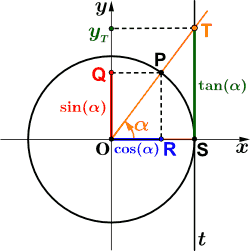
\includegraphics[width=150px]{images/trigon.png}\\
    $cos(x)=sin(x+\frac{\pi}{2})$\\
    $cos(x)^{2}+sin(x)^{2}=1$
\end{center}
parità: coseno è pari, infatti $cos(-x)=cos(x)$, mentre il seno è dispari perché $sin(-x)=-sin(x)$

\textbf{tangente e cotangente}\\la tangente, $tg(x)=\frac{sin(x)}{cos(x)}$, corrisponde alla lunghezza del segmento
che cade perpendicolare sull'asse delle x nel punto 1 e che interseca l'estensione del raggio. Il dominio della
tangente è $dom(tg)=\mathbb{R}/\{x=\frac{\pi}{2}+k\pi\mid k\in\mathbb{Z}\}$. La contangente,
$tg(x)=\frac{cos(x)}{sin(x)}$, invece cade sull'asse delle y nel punto 1.

Sia tangente e cotangente sono funzioni dispari e hanno periodo minimo in $\pi$

\textbf{Inverse}
\begin{center}
    $arcsin:[-1,1]\rightarrow[-\frac{\pi}{2},\frac{\pi}{2}]$\\
    $arcsin\doteq(sin\upharpoonright_{[-\frac{\pi}{2},\frac{\pi}{2}]})^{-1}$\\
    $arcsin(sin(x))=x \qquad \forall x\in[-\frac{\pi}{2},\frac{\pi}{2}]]$
\end{center}

\begin{center}
    $arccos:[-1,1]\rightarrow[0,\pi]$\\
    $arccos\doteq(cos\upharpoonright_{[0,\pi]})^{-1}$\\
    $arccos(cos(x))=x \qquad \forall x\in[0,\pi]$
\end{center}

\begin{center}
    $arctg:[-1,1]\rightarrow[-\frac{\pi}{2},\frac{\pi}{2}]$\\
    $arctg\doteq(tg\upharpoonright_{[-\frac{\pi}{2},\frac{\pi}{2}]})^{-1}$\\
    $arctg(tg(x))=x \qquad \forall x\in[-\frac{\pi}{2},\frac{\pi}{2}]]$
\end{center}

\begin{center}
    $arccotg:[-1,1]\rightarrow[0,\pi]$\\
    $arccotg\doteq(cotg\upharpoonright_{[0,\pi]})^{-1}$\\
    $arccotg(cotg(x))=x \qquad \forall x\in[0,\pi]$
\end{center}

\textbf{Esponenziali e logaritmi}\\Se $a>0, a^{x}\in\mathbb{R}$
\begin{center}
    $exp_{a}:\mathbb{R}\rightarrow\mathbb{R}$\\
    $\qquad\quad x\rightarrow a^{x}$
\end{center}
Se $a=1$ allora ho la funzione banale $a^{x}=1^{x}=1\quad \forall x\in\mathbb{R}$. Se $a\neq1$ allora $a^{x}>0$
quindi è limitato inferiormente e il minimo è 0.\\
L'esponenziale è bigiettiva, quindi invertibile, e la sua funzione inversa è il logaritmo
\begin{center}
    $a^{y}=x\qquad y=log_{a}(x)$
\end{center}
Dalle proprietà elementari determiniamo che
\begin{itemize}
    \item $log_{a}(a^{x})=x\qquad \forall x\in\mathbb{R}$
    \item $a^{log_{a}(x)}=x\qquad \forall x>0, x\in\mathbb{R}$
\end{itemize}

\textbf{Prop}\\Valgono le seguenti proprietà:
\begin{itemize}
    \item $log_{a}(x_{1}+x_{2})=log_{a}(x_{1})+log_{a}(x-{2})\qquad x_{1,2}>0$
    \item $log_{a}(x^{\alpha})=\alpha\cdot log_{a}(x)\qquad x>0, \alpha\in\mathbb{R}$
    \item $log_{b}(x)=log_{a}(x)\cdot log_{b}(a)\qquad x,a,b>0,a,b\neq 1$
\end{itemize}
Il logaritmo se viene indicato come $log$ è in base 10, mentre $ln$ se ha come base il numero di nepero

\newpage
\section{Successioni di numeri reali}
\begin{center}
    $a:\mathbb{N}\rightarrow\mathbb{R}$\\
    $n\in\mathbb{R}\rightarrow a(n)\in\mathbb{R}\qquad a(n)=a_{n}$\\
    $(a_{1},a_{2},a_{3},...,a_{n},a_{n+1},...)\Leftrightarrow (a_{n})(a_{n})_{n}(a_{n})_{n\in\mathbb{N}}$
\end{center}
I componenti della successione si chiamano \textbf{termini} della successione $(a_{n})$, mentre il valore $n$ si
dice \textbf{indice}.

NB: è importante \textbf{non confondere successione e immagine della successione}.\\Es: $(a_{n})=
    (2,-2,2,-2,2,-2,...)\qquad imm(a_{n})=\{2,-2\}$

Es: $\sqrt{2}$ si avvicina alla successione $a_{n+1}=\frac{a_{n}}{2}+\frac{1}{a_{n}}$ con $a_{n}>0$ e $a_{1}=2$.
La differenza tra $\sqrt{2}$ e $(a_{n}$, ossia $|a_{n}-\sqrt{2}|$ viene inteso come \textbf{errore assoluto}

\textbf{Def}\\Diremo che una successione \textbf{tende} o \textbf{converge} ad un certo numero reale $l$ se per
quanto piccolo si scelga $\varepsilon >0$ è possibile trovare un naturale $N$ per cui tutti i termini della
successione con indici $n<N$ approsimano $l$ con un errore minore di $\varepsilon$. In tal caso il numero $l$
si dice \textbf{limite} della successione e la convergenza viene descritta con il simbolo:
\begin{center}
    $a_{n}\to l\qquad\qquad n\to\infty$
\end{center}

La successione converge a $l\in\mathbb{R}$ se per ogni $\varepsilon>0$ esiste $N_{\varepsilon}\in\mathbb{N}$ tali
che:
\begin{center}
    $|a_{n}-l|<\varepsilon\qquad\forall n\in\mathbb{N}, n>N_{\varepsilon}$
\end{center}

Oss: le successioni per cui $a_{n}\to 0\qquad n\to\infty$ si dicono \textbf{infinitesime}

\textbf{Def - successioni divergenti}\\Una successione si dice avere limite a $+\infty$ o diverge a $+\infty$ e
scriveremo $a_{n}\to\infty\ quad n\to\infty$ quando, comunque scelto un numero reale, ogni termine della successione
da un certo indice in poi è maggiore del numero reale scelto.\\In modo formale, per ogni $M\in\mathbb{R}$ esiste
$N_{M}\in\mathbb{N}$ tali che per ogni $n>N_{M}$ si ha $a_{n}>M$. Lo stesso si può fare nel caso $(a_{n})$ diverge
a $-\infty$. Ossia posso dire che $(-a_{n})$ diverge a $+\infty$, per cui vale la definizione di prima, ossia,
per ogni scelta di $M\in\mathbb{R}$ trovo $N_{M}\in\mathbb{N}$ per cui ogni $n>N_{M}\quad -a_{n}>M$ ossia
$A_{n}<-M$. Anche ora si può scrivere $a_{n}\to-\infty\quad n\to\infty$

\textbf{Def - Carattere delle successioni}\\Sia $(a_{n})$ successione reale. Se $(a_{n})$ ammette limite (finito
o infinito) diremo che la successione $(a_{n})$ è \textbf{regolare}. Se non ammette limite diremo che la
successione è \textbf{irregolare} o \textbf{indeterminata}. Stabilire se $(a_{n})$ è regolare o indeterminata vuol
dire stabilire il carattere della succesione.

\textbf{Teorema - Unicità del limite}\\Ogni successione reale regolare ha un solo limite

\textbf{Definizione topologica di limite}\\Concetto di intorno\\$I_{\varepsilon}(l)\doteq(l-\varepsilon,
l+\varepsilon)\Rightarrow$ Intorno simmetrico di raggio $\varepsilon>0$.\\Al variare di $\varepsilon>0$ considero la
    famiglia degli intorni simmetrici
    \begin{center}
        $\mathcal{B}_{l}\doteq\{I_{\varepsilon}(l)\mid\varepsilon>0\}$
    \end{center}
$\mathcal{B}_{l}$ è detta \textbf{base di intorni} di $l\in\mathbb{R}$. Posso verificare gli intorni di $\pm\infty$
    come gli intervalli $(M,+\infty)$ oppure $(-\infty,M)$ per ogni scelta di $M\in\mathbb{R}$

    \textbf{Teorema - Cambiamento delle variabili}\\Sia $f:\mathbb{N}\to\mathbb{N}$ strettamente crescente. Allora se
$(a_{n})$ è regolare vale:
    \begin{center}
        $lim\ a_{n}=lim\ a_{f(n)}$
    \end{center}

    Corollario:\\Per ogni $k\in\mathbb{N}$ finito ho:
    \begin{center}
        $lim\ a_{n+k}=lim\ a_{n}$
    \end{center}

    \textbf{Proprietà delle successioni regolari\\Limitatezza}
    \begin{center}
        $a:\mathbb{N}\to\mathbb{R}$\\
        $a(\mathbb{N})\subset\mathbb{R}$\\
        $a(\mathbb{N})=\{a_{n}\mid n\in\mathbb{N}\}$
    \end{center}
    Diremo che $(a_{n})$ è \textbf{superiormente limitata} se $a(\mathbb{N})$ lo è, ossia esiste $M\in\mathbb{R}$ tale che
$a_{n}<M\ \forall n\in\mathbb{N}$, e quindi diremo che accetta estremo superiore. Invece $(a_{n})$ è
    \textbf{inferiormente limitata} se $a(\mathbb{N})$ lo è, ossia esiste $m\in\mathbb{R}$ tale che $a_{n}>m\ \forall
n\in\mathbb{N}$, e quindi accetta estremo inferiore. Diremmo che $(a_{n})$ è \textbf{limitata} se lo è sia
    inferiormente che superiormente

    \textbf{Prop}\\Ogni successione convergente è limitata. Ogni successione divergente positivamente è inferiormente
    limitata e ogni successione divergente negativamente è superiormente limitata

    \textbf{Prop}\\Se $(a_{n})$ è regolare allora $(|a_{n}|)$ è reoglare. Se $(|a_{n}|)$ è infinitesima allora $(a_{n})$
    è infinitesima

    \textbf{Monotonia\\Def}\\Sia $(a_{n})$ successione reale.
    \begin{itemize}
        \item $(a_{n})$ è crescente se $a_{n}\leq a_{n+1}\quad\forall n$
        \item $(a_{n})$ è decrescente se $a_{n}\geq a_{n+1}\quad\forall n$
        \item $(a_{n})$ è strettamente crescente se $a_{n}< a_{n+1}\quad\forall n$
        \item $(a_{n})$ è strettamente decrescente se $a_{n}> a_{n+1}\quad\forall n$
    \end{itemize}

    \textbf{Teorema}\\Ogni successione monotona è regolare. in particolare se monotona crescente allora
$lim\ a_{n}=inf(a_{n})$

    \textbf{Algebra dei limiti}
    \begin{center}
        $\overline{\mathbb{R}}\doteq\{-\infty\}\cup\mathbb{R}\cup\{+\infty\}$\\
        $x\in\overline{\mathbb{R}}\qquad -\infty\leq x\leq +\infty$
    \end{center}
    Relazioni indeterminate:
    \begin{itemize}
        \item $\pm\infty\mp\infty$
        \item $0\cdot\pm\infty$
        \item $\frac{0}{0},\frac{\pm\infty}{\pm\infty}$
        \item $0^{0}, +\infty^{0},1^{\pm\infty}$
    \end{itemize}
    \begin{center}
        $a\in\mathbb{R}\qquad  a+\pm\infty=\pm\infty\qquad  +\infty^{a}=+\infty$

        $a\in\mathbb{R_{+}}\qquad a\cdot\pm\infty=\pm\infty$

        $b\in\mathbb{R_{-}}\qquad b\cdot\pm\infty=\mp\infty\qquad +\infty^{b}=0$

        $+\infty+\infty=+\infty\qquad-\infty-\infty=-\infty$

        $\frac{1}{\pm\infty}=0\qquad+\infty^{-\infty}=0$
    \end{center}

    \textbf{Prop}\\Supponiamo $(a_{n})$ regolare con $a_{n}\to l\in\overline{\mathbb{R}}$.
    \begin{enumerate}
        \item Se $l_{0}\in\mathbb{R}$ è tale che
              \begin{center}
                  $lim\ a_{n}=l>l_{0}$
              \end{center} allora esistono un $N\in\mathbb{N}$ e un numero
              reale $s>0$ tali che
              \begin{center}
                  $a_{n}>s\qquad\forall n>N$
              \end{center}
        \item Se $l_{0}\in\mathbb{R}$ è tale che
              \begin{center}
                  $lim\ a_{n}=l<l_{0}$
              \end{center}
              Allora esistono $N\in\mathbb{N}$ ed un numero reale $s<l_{0}$ tali che
              \begin{center}
                  $a_{n}<s\qquad\forall n>N$
              \end{center}
    \end{enumerate}

    Corollario\\Sia $(a_{n})$ convergente a $l\neq 0$. Allora:
    \begin{itemize}
        \item Se $l>0$ esiste $N\in\mathbb{N}$ tale che $a_{n}>\frac{l}{2}\quad\forall n>N$
        \item Se $l<0$ esiste $N\in\mathbb{N}$ tale che $a_{n}<\frac{l}{2}\quad\forall n>N$
        \item Esiste $N\in\mathbb{N}$ tale che $|a_{n}|>\frac{|l|}{2}\quad\forall n>N$
    \end{itemize}

    \textbf{Teorema - Algebra delle somme}\\Siano $(a_{n}),(b_{n})$ successioni regolari, allora:
    \begin{enumerate}
        \item $\ $
              \begin{center}
                  $lim\ (a_{n}+b_{n})=lim\ a_{n} + lim\ b_{n}\qquad$
              \end{center}
              qualora il secondo membro sia ben definito in $\overline{\mathbb{R}}$
        \item $\ $
              \begin{center}
                  $lim\ (a_{n}-b_{n})=lim\ a_{n} - lim\ b_{n}\qquad$
              \end{center}
              qualora il secondo membro sia ben definito in $\overline{\mathbb{R}}$
    \end{enumerate}

    \textbf{Teorema - Prodotto di limiti per infinitesima}\\Siano $(a_{n})$ infinitesima e $(b_{n})$ limitata. Allora
$a_{n}\cdot b_{n}\to 0$ è infinitesima

    \textbf{Teorema - Algebra dei prodotti}\\Siano $(a_{n}),(b_{n})$ regolari. Allora si ha:
    \begin{center}
        $lim\ (a_{n}\cdot b_{n})=lim\ a_{n}\cdot lim\ b_{n}$
    \end{center}
    qualora in secondo membro sia ben definito in $\overline{\mathbb{R}}$

    \textbf{Teorema - Limite dei reciproci}\\Sia $(a_{n})$ regolare $a_{n}\to a\in\overline{\mathbb{R}}$. Sia hanno i
    seguenti casi:
    \begin{itemize}
        \item Se $a_{n}\neq 0\quad\forall n\in\mathbb{N}$ e $a\neq 0$ allora \begin{center}
                  $\frac{1}{a_{n}}\to\frac{1}{a}$
              \end{center}
        \item Se $a=0$ e $a_{n}>0\quad\forall n\in\mathbb{N}$ allora \begin{center}
                  $\frac{1}{a_{n}}\to+\infty$
              \end{center}
        \item Se $a=0$ e $a_{n}<0\quad\forall n\in\mathbb{N}$ allora \begin{center}
                  $\frac{1}{a_{n}}\to-\infty$
              \end{center}
    \end{itemize}

    \textbf{Teorema - Algebra dei rapporti}\\Supponiamo $(a_{n})(b_{n})$ regolari. Allora se $b_{n}\neq 0\quad\forall
n\in\mathbb{N}$ si ha \begin{center}
        $lim\ \frac{a_{n}}{b_{n}}=\frac{lim\ a_{n}}{lim\ b_{n}}$
    \end{center}
    qualora il secondo membro sia ben definito in $\overline{\mathbb{R}}$

    Corollario
    \begin{center}
        $lim\ R(a_{n})=lim\ \frac{P(a_{n})}{Q(a_{n})}=\frac{lim\ P(a_{n})}{lim\ Q(b_{n})}=\frac{P(a)}{Q(a)}=R(a)$
    \end{center}

    \textbf{Lemma}\\Consideriamo le successioni $(e_{n}),(E_{n})$ di termini generici:
    \begin{center}
        $e_{n}=(1+\frac{1}{n})^{n}\qquad E_{n}=(1+\frac{1}{n})^{n+1}$
    \end{center}
    Sono vere le seguenti affermazioni:
    \begin{enumerate}
        \item $1<e_{n}<E_{n}\quad\forall n\in\mathbb{N}$
        \item $(e_{n})$ è strettamente crescente
        \item $(E_{n})$ è strettamente decrescente
    \end{enumerate}

    \textbf{Def - Numero di Nepero}
    \begin{center}
        $e\cdot lim\ (1+\frac{1}{n})^{n}$
    \end{center}

    \textbf{Def}\\Sia $f:A\subseteq\mathbb{R}\to\mathbb{R},\ a\in A$. Allora diremmo che $f$ è \textbf{CPS} in a se per
    ogni successione $(a_{n}), con a_{n}\in A\quad\forall n\in\mathbb{N}$, convergente ad a si ha
    \begin{center}
        $lim\ f(a_{n})=f(a)$
    \end{center}
    Se tale proprietà vale $\forall a\in A$ diremo che $f$ è CPS (in $A$)

    Oss: Definizione poco pratica\\$lim\ f(a_{n})=f(lim\ a_{n})$\\$A\subseteq dom(f)$

    \textbf{Lemma}\\Sono CPS nei loro domini naturali le seguenti funzioni
    \begin{itemize}
        \item la funzione identica $id$
        \item funzioni affini: $a\in\mathbb{R}\quad F:\mathbb{R}\to\mathbb{R}\quad F(x)\doteq x+a$
        \item valore assoluto
        \item polinomi e razionali
        \item la funzione reciproca: $x\to\frac{1}{x}$
        \item potenze razionali: $x\to x^{t}$ con $t\in\mathbb{Q}$
    \end{itemize}

    \textbf{Confronti e stime asintotiche}

$a_{n}\qquad(b_{n})$

$a_{n}\to\pm\infty\qquad b_{n}\to\pm\infty$\\
$lim\ \frac{a_{n}}{b_{n}}=\begin{cases}
    0                    & \rightarrow  (a_{n})$ è infinito di ordine inferiore di $(b_{n}) \\
    l\in\mathbb{R}/\{0\} & \rightarrow (a_{n})$ ha lo stesso ordine d'infinito di $(b_{n}   \\
    \pm\infty            & \rightarrow  (a_{n})$ è infinito di ordine maggiore di $(b_{n}   \\
    \nexists             & \rightarrow  $non posso dire nulla$
\end{cases}$

$a_{n}\to 0\qquad b_{n}\to 0$\\
$lim\ \frac{a_{n}}{b_{n}}=\begin{cases}
    \pm\infty            & \rightarrow (a_{n})$ è infinitesimo di ordine inferiore di $(b_{n}) \\
    l\in\mathbb{R}/\{0\} & \rightarrow (a_{n})$ è infinitesimo dello stesso ordine di $(b_{n}  \\
    0                    & \rightarrow (a_{n})$ è infinitesimo di ordine maggiore di $(b_{n}   \\
    \nexists             & \rightarrow $non posso dire nulla$
\end{cases}$

    Con $lim\ \frac{a_{n}}{b_{n}}=1$ dirò che $(a_{n})$ è \textbf{asintotica} a $(b_{n})$ e indicheremo con il simbolo
$(a_{n})\sim(b_{n})$

    \textbf{Prop}\\Valgono i seguenti fatti:
    \begin{itemize}
        \item Se $a_{n}\sim B_{n}$, le successioni hanno lo stesso carattere
        \item Se $a_{n}\sim b_{n}\sim ... \sim c_{n}\Rightarrow a_{n}\sim b_{n}$
        \item una espressione composta da un prodotto o quoziente di più fattori può essere stimata fattore per fattore:
              \begin{center}
                  $a_{n}\sim a_{n}^{I}\quad b_{n}\sim b_{n}^{I}\quad c_{n}\sim c_{n}^{I}\Rightarrow \frac{a_{n}b_{n}}{c_{n}}
                      \sim\frac{a_{n}^{I}b_{n}^{I}}{c_{n}^{I}}$
              \end{center}
    \end{itemize}

    \textbf{Teorema - Criterio del rapporto}\\Sia $(a_{n})$ con $a_{n}>0\quad n\in\mathbb{N}$. Se esiste
    \begin{center}
        $lim\ \frac{a_{n+1}}{a_{n}}=l\in\overline{\mathbb{R}}$
    \end{center}
    allora
    \begin{itemize}
        \item Se $l<1\Rightarrow a_{n}\to 0$
        \item Se $l>1\ ($incluso $l=+\infty)\Rightarrow a_{n}\to +\infty$
        \item Se $l=1$ non posso dire nulla
    \end{itemize}
    65

    \textbf{Teorema - Gerarchia degli infiniti}\\Vale la seguente lista di risultati:
    \begin{enumerate}
        \item $lim\ \frac{log_{a}n}{n^{\alpha}}=0\qquad\forall a>1,\forall\alpha>0$
        \item $lim\ \frac{n^{\alpha}}{a^{n}}=0$
        \item $lim\ \frac{a^{n}}{n!}=0$
        \item $lim\ \frac{n!}{n^{n}}=0$
    \end{enumerate}

$+\infty^{0}=lim\ \sqrt[n]{n}=lim\ n^{\frac{1}{n}}=lim\ e^{\frac{1}{n}log(n)}=e^{0}=1$

$0<x=e^{log(x)}=a^{log_{a}(x)}$

    \textbf{Formula di Stirling}
    \begin{center}
        $n!\sim\sqrt{2\pi n}\cdot n^{n}e^{-n}$
    \end{center}

    \newpage
    \section{Limiti di funzioni}
    \textbf{Def}\\Si dice che
    \begin{center}
        $lim\ f(x)=l$\\
        $x\to c\qquad\qquad$\\
        $x\in\mathbb{I}\qquad\qquad$
    \end{center}
    Se per ogni successione $(x_{n})$ con $x_{n}\in\mathbb{I},\ \forall n\in\mathbb{N}$ per cui $x_{n}
\to c\ n\to\infty\ \Rightarrow f(x_{n})\to lo\quad n\to+\infty$

    Con $c\in\overline{\mathbb{R}}$:
    \begin{itemize}
        \item Se $c\in\mathbb{R}\qquad U_{c}(\delta)=(c-\delta,c+\delta)$
        \item se $c=\pm\infty\qquad U_{\pm\infty}(\delta)=(\delta,+\infty)$ oppure $(-\infty,\delta)$
    \end{itemize}

    \textbf{Def}\\Diremo che una funzione $f$ ha una certa proprietà \textbf{definitivamente} per $x\to c$
    se esiste un intorno $U$ di $c$ tale che la proprietà di $f^{(x)}$ vale per ogni $x\in U,\ x\neq c$

    \textbf{Def - Limite in senso topologico}\\Sia $c\in\overline{\mathbb{R}}$ e sia $f$ una funzione
    definita almeno definitivamente per $x\to c$. Si dice che
    \begin{center}
        $lim_{x\to c}f(x)=l\in\overline{\mathbb{R}}$
    \end{center}
    se per ogni intorno $U_{l}$ esiste un intorno di $c,\ V_{c}$ tali che per ogni $x\in V_{c},\ x\neq c$,
    allora $f(x)\in U_{l}$

    \textbf{Teorema - Teorema del ponte}\\Siano $f:I\to\mathbb{R}$, $I$ intervallo di $\mathbb{R}$ non
    degenere, $l\in\overline{\mathbb{R}},\ c\in\overline{\mathbb{R}}$ allora
    \begin{center}
        $lim_{x\to c}f(x)=l$
    \end{center}
    se e solo se per ogni successione $(x_{n})$ per cui $x_{n}\in I$ con $x_{n}\neq c\quad\forall n\in
\mathbb{N}$ per cui $x_{n}\to c\quad n\to+\infty\Rightarrow f(x_{n})\to l\quad n\to+\infty$
    \newpage
    4 possibilità caratterizzate dalla scelta di $c$ e $l$\\
    \textbf{Limite finito all'infinito}
    \begin{center}
        $lim_{x\to c}f(x)=l$
    \end{center}
    \subitem $c=+\infty, l\in\mathbb{R}$.\\$\forall\varepsilon>0 \exists K>0$ tali che $\forall x$ per
cui $x>K$ allora $|f(x)-l|<\varepsilon$
\subitem $c=-\infty, l\in\mathbb{R}$.\\$\forall\varepsilon>0 \exists K>0$ tali che $\forall x$ per
    cui $x<-K$ allora $|f(x)-l|<\varepsilon$

    Queste tipologie di limite caratterizza le cosidette rette asintotiche orizzontali o
    \textbf{asintoti orizzontali} delle funzioni

    \textbf{Def}\\Se $l\in\mathbb{R}\ c\in\overline{\mathbb{R}}$ si dice che
    \begin{center}
        $lim_{x\to c}f(x)=l^{+}\qquad$ (rispettivo $l^{-}$)
    \end{center}
    se per ogni successione $(x_{n})$ con $x_{n}\in I\ x_{n}\neq c$ e $x_{n}\to c\quad n\to+\infty$
    si ha che $f(x_{n})\to l^{+}$ per $n\to+\infty$ se e solo se $f(x_{n})\geq l$ definitivamente
    (convergenza per \textbf{eccesso} ($l^{+}$) o per \textbf{difetto}($l^{-}$))

    \textbf{Limite finito all'infinito}
    \begin{center}
        $lim_{x\to c}f(x)=l$
    \end{center}
    \subitem $c=+\infty, l=+\infty$.\\$\forall H>0 \exists K>0$ tali che $\forall x$ per
cui $x>K$ allora $f(x)>H$
\subitem $c=+\infty, l=-\infty$.\\$\forall H>0 \exists K>0$ tali che $\forall x$ per
    cui $x>K$ allora $f(x)>-H$
    \subitem $c=-\infty, l=+\infty$.\\$\forall H>0 \exists K>0$ tali che $\forall x$ per
cui $x<-K$ allora $f(x)>H$
\subitem $c=-\infty, l=-\infty$.\\$\forall H>0 \exists K>0$ tali che $\forall x$ per
    cui $x<-K$ allora $f(x)<-H$

    Può accadere che in questi casi esistono \textbf{asintoti obliqui}

    \textbf{Def}\\Si dice che la funzione $f$ ha asintoto obliquo di equazione $y=mx+q\quad m\neq 0$ per
$x\to+\infty\ (x\to-\infty)$ se accade che
    \begin{center}
        $lim_{x\to+\infty}(f(x)-(mx+q))=0\qquad(lim_{x\to-\infty}(f(x)-(mx+q))=0)$
    \end{center}

    \textbf{Prop}\\La funzione $f$ ammette asintoto obliquo per $x\to+\infty$ se e solo se valgono
    le seguenti condizioni:
    \begin{itemize}
        \item $lim_{x\to+\infty}\frac{f(x)}{x}=m\neq 0$
        \item $lim_{x\to+\infty}(f(x)-mx)=q$
    \end{itemize}

    \textbf{Limite infinito al finito}
    \begin{center}
        $lim_{x\to c}f(x)=l$
    \end{center}
    \subitem $c\in\mathbb{R}, l=+\infty$.\\$\forall H>0 \exists \delta>0$ tali che $\forall x$ per
cui $0<|x-c|<\delta$ allora $f(x)>H$
\subitem $c\in\mathbb{R}, l=-\infty$.\\$\forall H>0 \exists \delta>0$ tali che $\forall x$ per
    cui $0<|x-c|<\delta$ allora $f(x)<-H$

    Si possono specificare nel caso in cui $c\in\mathbb{R}$ i limiti destro e sinistro:
    \begin{itemize}
        \item $lim_{x\to c^{+}}f(x)=l$ per cui $x>c$
        \item $lim_{x\to c^{-}}f(x)=l$ per cui $x<c$
    \end{itemize}

    \textbf{Def}\\Si dice che $f$ ha \textbf{asintoto verticale} di equazione $x=c\in\mathbb{R}$ se accade
    che
    \begin{center}
        $lim_{x\to c}f(x)=+\infty$ oppure $lim_{x\to c}f(x)=-\infty$
    \end{center}
    o rispettivamente a seconda dei casi
    \begin{center}
        $lim_{x\to c^{+}}f(x)=+\infty$ oppure $lim_{x\to c^{+}}f(x)=-\infty$\\
        $lim_{x\to c^{-}}f(x)=+\infty$ oppure $lim_{x\to c^{-}}f(x)=-\infty$
    \end{center}

    \textbf{Limite finito al finito}
    \begin{center}
        $lim_{x\to c}f(x)=l$
    \end{center}
$\forall\varepsilon>0 \exists\delta>0$ tale che per ogni $x$ per cui $0<|x-c|<\delta$ allora
    \begin{center}
        $|f(x)-l|<\varepsilon$
    \end{center}

    \textbf{Def}\\Diremo che $c$ è un \textbf{punto di discontinuità} per la funzione $f$ quando i limiti
    destro e sinistro di $f$ per $x\to c$ esistono e sono diversi
    \begin{center}
        $lim_{x\to c^{+}}f(x)-lim_{x\to c^{-}}f(x)=$ salto di $f$ in $c$
    \end{center}

    NB: $lim_{x\to+\infty}sin(x)$ non esiste

    \textbf{Calcolo dei limiti}\\\textbf{Teorema - Criterio del confronto}\\ Se per $x\to c$ ho $f(x)\to l$, $g(x)\to l$
    e si ha che vale $f(x)\leq h(x)\leq g(x)$ definitivamente per $x\to c$ allora $h(x)\to l$ per $x\to c$

    Corollario\\Se per $x\to c$ si ha $g(x)\to 0$ e $|h(x)|\leq g(x)$ definitivamente per $x\to c$ allora $h(x)\to 0$
    per $x\to c$

    Corollario\\Se $f(x)\to 0\ x\to c$ e $g(x)$ è limitata definitivamente per $x\to c$ allora $f(x)g(x)\to 0\quad
x\to c$

    \textbf{Teorema - Permanenza del segno}
    \begin{itemize}
        \item Se $f(x)\to l>0$ per $x\to c$ allora si ha che $f(x)>0$ definitivamente per $x\to c$
        \item se $f(x)\to l$ e $f(x)\geq 0$ per $x\to c$ allora $l\geq 0$
        \item Se $f$ è asintotica in $c$ e $f(c)>0$ allora $f(x)>0$ definitivamente per $x\to c$
    \end{itemize}

    \textbf{Teorema - Algebra dei limiti}\\Se $f$ e $g$ sono due funzoini definite almeno rispettivamente per $x\to c$
    e $f(x)\to l_{1}$ e $g(x)\to l_{2}$ per $x\to c$ allora
    \begin{center}
        $f\pm g=l_{1}\pm l_{2}\quad x\to c$\\
        $f\cdot g=l_{1}\cdot l_{2}\quad x\to c$\\
        $\frac{f}{g}=\frac{l_{1}}{l_{2}}\quad x\to c$
    \end{center}

    \textbf{Teorema - Cambio delle variabili}\\Siano $f,g$ funzioni tali che sia ben definito $f\circ g$ almeno
    definitivamente per $x\to x_{0}\in\overline{\mathbb{R}}$ e supponiamo che
    \begin{itemize}
        \item $g(x)\to t_{0}$ per $x\to x_{0}$ con $g(x)\neq t_{0}$ definitivamente per $x\to x_{0}$
        \item esiste $lim_{t\to t_{0}}f(t)=l\in\overline{\mathbb{R}}$
    \end{itemize}
    Allora $lim_{x\to x_{0}}f(g(x))= lim_{t\to t_{0}}f(t)$

    \textbf{Limiti notevoli}
    \begin{center}
        \begin{tabular}{l c c}
            $lim_{x\to 0}\frac{sin(x)}{x}$           & $\Rightarrow$ & $1$           \\
            $lim_{x\to 0}\frac{1-cos(x)}{x^{2}}$     & $\Rightarrow$ & $\frac{1}{2}$ \\
            $lim_{x\to 0}\frac{tg(x)}{x}$            & $\Rightarrow$ & $1$           \\
            $lim_{x\to 0}\frac{arcsin(x)}{x}$        & $\Rightarrow$ & $1$           \\
            $lim_{x\to 0}\frac{arctg(x)}{x}$         & $\Rightarrow$ & $1$           \\
            $lim_{x\to\pm\infty}(1+\frac{1}{x})^{x}$ & $\Rightarrow$ & $e$           \\
            $lim_{x\to 0}\frac{log(1+x)}{x}$         & $\Rightarrow$ & $1$           \\
            $lim_{x\to 0}\frac{e^{x}-1}{x}$          & $\Rightarrow$ & $1$           \\
        \end{tabular}
    \end{center}

    \textbf{Def - Prolungamento per continuità}\\Se $f$ non è definità in $x=c$ ma esiste
    \begin{center}
        $lim_{x\to c}f(x)=l\in\mathbb{R}$
    \end{center}
    allora la funzione può essere \textbf{estesa per continuità} ponendo $f(c)\doteq l$
    \begin{center}
        $\tilde{f}(x)=
            \begin{cases}
                f(x) & x\neq c \\
                l    & x=c
            \end{cases}$
    \end{center}

    \textbf{Confronti e stime asintotiche\\Def}\\Si dice che 2 funzioni $f,g$ sono \textbf{asintotiche} per $x\to c$ se
    \begin{center}
        $lim_{x\to c}\frac{\hat{f}(x)}{g(x)}=1$
    \end{center}
    e si scrive $f\sim g$

    \textbf{Teorema - Gerarchia degli infiniti}\\
    \text{Si possono dimostrare i seguenti limiti validi per $\alpha,\beta>0\quad a,b>1,\delta$ qualunque}
    \begin{enumerate}
        \item $lim_{x\to+\infty}\frac{(log_{a}(x))^{\alpha}}{x^{\beta}}=0$
        \item $lim_{x\to+\infty}\frac{x^{\beta}}{b^{x}}=0$
        \item $lim_{x\to 0^{+}}x^{\beta}(-log(x))^{\delta}=0$
    \end{enumerate}

    \section{Limiti e tecnologia dell'o piccolo}
    \textbf{Def}\\\text{Si dice che $f$ è \textbf{o piccolo} di $g$ per $x\to x_{0}$ e  si scrive}
    \begin{center}
        $f(x)=o(g(x))\quad x\to x_{0}$
    \end{center}
    \text{se esiste una fuzione $w(x)$ tale che}
    \begin{center}
        $f(x)=w(x)g(x)$\\
        $lim_{x\to x_{0}}w(x)=0$
    \end{center}

    \textbf{Def - Quasi equivalente}\\
    \text{
        supponiamo che $g(x)\neq 0$ almeno definitivamente in $x_{0}\in\overline{\mathbb{R}}$ allora
    }
    \begin{center}
        $w(x)=\frac{f(x)}{g(x)}\Rightarrow lim_{x\to x_{0}}\frac{f(x)}{g(x)}=0$
    \end{center}

    \textbf{Proprietà algebriche dell'o piccolo}\\
$f_{1}(x)=o(g(x))\quad x\to x_{0}\qquad f_{2}(x)=o(g(x))\quad x\to x_{0}$

    \begin{itemize}
        \item $f_{1}+f_{2}:$
              \subitem $f_{1}(x)+f_{2}(x)=w_{1}(x)g(x)+w_{2}(x)g(x)=g(x)(w_{1}(x)+w_{2}(x))$

              quindi\\
              $o(g(x))+o(g(x))=o(g(x))\qquad x\to x_{0}$
        \item $f_{1}-f_{2}:$
              \subitem $f_{1}(x)+f_{2}(x)=g(x)(w_{1}(x)-w_{2}(x))$

              $o(g(x))-o(g(x))=o(g(x))\qquad x\to x_{0}$
        \item $cf_{1}$
              \subitem $cf_{1}(x)=cw_{1}(x)g(x)$

              $c\cdot o(g(x))=o(g(x))\qquad x\to x_{0}$
        \item $f_{1}\cdot f_{2}$
              \subitem $f_{1}(x)f_{2}(x)=w_{1}(x)w_{2}(x)g^{2}(x)$

              $o(g(x))\cdot o(g(x))=o(g^{2}(x))\qquad x\to x_{0}$
        \item $\frac{f_{1}}{f_{2}}$
              \subitem $\frac{f_{1}(x)}{f_{2}(x)}=\frac{w_{1}}{w_{2}}=\frac{0}{0}=?$

    \end{itemize}

    \textbf{Transitività di o piccolo}\\Se $f(x)=o(g(x))\quad x\to x_{0}$ e $g(x)=o(h(x))\quad x\to x_{0}$ allora
    \begin{center}
        $f(x)=o(h(x))\quad x\to x_{0}$
    \end{center}
    \textbf{altre proprietà}

$f(x)=o(g_{1}(x)+g_{2}(x))=o(g_{1}(x))+o(g_{2}(x))$

$f(x)=o(c\cdot g(x))=o(g(x))$

    \textbf{Teorema - Cancellazione}\\Se $f_{1}(x)=o(f(x))\quad g_{1}(x)=o(g(x))$
    \begin{center}
        $lim_{x\to x_{0}}\frac{f(x)+f_{1}(x)}{g(x)+g_{1}(x)}=lim_{x\to x_{0}}\frac{f(x)}{g(x)}$
    \end{center}

    \textbf{Sviluppi per $x\to 0$}
    \begin{center}
        \begin{tabular}{l c c | l c c}
            $sin(x)$ & $0$ & $x+o(x)$   & $arctg(x)$  & $=$ & $x+o(x)$                 \\
            $tg(x)$  & $0$ & $x+o(x)$   & $arcsin(x)$ & $=$ & $x+o(x)$                 \\
            $cos(x)$ & $0$ & $1+o(x)$   & $cos(x)$    & $=$ & $1-\frac{x^{2}}{2}+o(x)$ \\
            $e^{x}$  & $0$ & $1+x+o(x)$ & $log(1+x)$  & $=$ & $x+o(x)$
        \end{tabular}
    \end{center}

    Oss: $x^{\alpha}=o(x^{\beta})\quad \forall \alpha>\beta\quad x\to 0$

    \textbf{Def - Equivalenza asintotica}\\Si di che $f$ è \textbf{asintoticamente equivalente} a $g$ per $x\to 0$
    e si scrive $f(x)\sim g(x)\quad x\to x_{0}$ se esiste una funzione $w$ tale che
    \begin{center}
        $f(x)=w(x)g(x)$\\
        con\\
        $lim_{x\to x_{0}}w(x)=1$
    \end{center}

    \textbf{Def - Quasi equivalente}\\ Se $g(X)\neq 0$ definitivamente per $x\to x_{0}$ (tranne al più di $x$) allora
$f(x)\sim g(x)\quad x\to x_{0}$ se
    \begin{center}
        $lim_{x\to x_{0}}\frac{f(x)}{g(x)}=1$
    \end{center}

    \newpage
    \section{Derivabilità e differenziabilità}
    \textbf{Def}\\Si dice che $f$ è \textbf{differenziabile} in $x_{0}$ se esiste $\alpha\in\mathbb{R}$ tale che
    \begin{center}
        $f(x_{0}+h)=f(x_{0})+\alpha h+o(h)\quad h\to 0$
    \end{center}
    In tal caso $\alpha$ è detto \textbf{differenziale} di $f$ in $x_{0}$

    \textbf{Teorema}\\Una funzione $f$ è differenziale in $x_{0}$ se e solo se $f$ è derivabile in $x_{0}$. Inoltre,
    se questo è vero, allora $\alpha=f^{I}(x_{0})$

    \textbf{Teorema}\\Ogni funzione $f$ derivabile in $x_{0}$ è continua in $x_{0}$

    \textbf{Regole della derivazione e derivate di funzioni elementari}
    \begin{center}
        \begin{tabular}{l c c | l c c}
            $($costante$)^{I}$ & $=$ & $0$                 & $(arctg(x))^{I}$   & $=$ & $\frac{1}{1+x^{2}}$                     \\
            $(e^{x})^{I}$      & $=$ & $e^{x}$             & $(arcsin(x))^{I}$  & $=$ & $\frac{1}{\sqrt{1-x^{2}}}$              \\
            $(a^{x})^{I}$      & $=$ & $a^{x}\cdot log(a)$ & $(arccos(x))^{I}$  & $=$ & $-\frac{1}{\sqrt{1-x^{2}}}$             \\
            $(log(x))^{I}$     & $=$ & $\frac{1}{x}$       & $(tg(x))^{I}$      & $=$ & $\frac{1}{cos^{2}(x)}=1+tg^{2}(x)$      \\
            $(sin(x))^{I}$     & $=$ & $cos(x)$            & $(x^{\alpha})^{I}$ & $=$ & $\alpha x^{\alpha-1}\quad,\alpha\neq 0$ \\
            $(cos(x))^{I}$     & $=$ & $-sin(x)$           &                    &     &                                         \\
        \end{tabular}

        \begin{tabular}{l c c | l c c}
            $(f\pm g)^{I}$      & $=$ & $f^{I}\pm g^{I}$              & $(\alpha f)^{I}$    & $=$ & $\alpha f^{I}$              \\
            $(f\cdot g)^{I}$    & $=$ & $f^{I}g +f g^{I}$             & $(\frac{1}{f})^{I}$ & $=$ & $-\frac{f^{I}}{f^{2}}$      \\
            $(\frac{f}{g})^{I}$ & $=$ & $\frac{f^{I}g-fg^{I}}{g^{2}}$ & $(f(g(x)))^{I}$     & $=$ & $f^{I}(g(x))\cdot g^{I}(x)$ \\
        \end{tabular}
        \begin{center}
            $(f(x))^{g(x)}=f^{g}(g^{I}ln(f)+\frac{g+f^{I}}{f})$
        \end{center}

        Se $f$ e $g$ sono inverse una dell'altra: $g^{I}(x)=\frac{1}{f^{I}(g(x))}$

    \end{center}

    \newpage
    \section{De L'Hôpital e Taylor}
    \textbf{Teorema di de l'hopital}
    \begin{center}
        $lim_{x\to x_{0}}\frac{f(x)}{g(x)}$
    \end{center}
    Supponiamo che
    \begin{itemize}
        \item Al netto delle condizione sopra le quali i rapporti $\frac{f}{g}>\frac{f^{I}}{g^{I}}$ esistono in un
              opportuno intorno di $x_{0}$
        \item il limite sia del tipo $\frac{0}{0},\frac{\pm\infty}{\pm\infty}$
        \item esiste in $\overline{\mathbb{R}}$ il limite
              \begin{center}
                  $lim_{x\to x_{0}}\frac{f^{I}(x)}{g^{I}(x)}$
              \end{center}
    \end{itemize}
    allora
    \begin{center}
        $lim_{x\to x_{0}}\frac{f(x)}{g(x)}=lim_{x\to x_{0}}\frac{f^{I}(x)}{g^{I}(x)}$
    \end{center}

    Operativamente: eseguo il limite e controllo che sia del tipo indefinito, poi eseguo il limite delle derivate. Se
    quest'ultimo non esiste, non posso dire nulla del primo limite. Se esiste in $\overline{\mathbb{R}}$, tutto ok.
    Se è ancora del tipo indeterminato allora riapplico l'hopital

    \textbf{Teorema di Taylor}\\Possiamo approssimare una funzione $f(x)$ con un polinomio $P_{n}(x)$ di grado $P\leq n$
    con $n\in\mathbb{N}$ tale che
    \begin{center}
        $f(x)=P_{n}(x)+o(x^{n})\quad x\to 0$
    \end{center}

    Sia $\delta>0$ e sia $f:(-\delta,\delta)\to \mathbb{R}$. Sia $n\in\mathbb{N}$ e supponiamo che
    \begin{itemize}
        \item $f$ è derivabile in $(-\delta,\delta)\ n-1$ volte
        \item $f$ è derivabile $n$-volte in $x=0$
    \end{itemize}
    Allora esiste il polinoimo di Taylor $P_{n}(x)$ ed è dato dalla seguente formula
    \begin{center}
        $P_{n}(x)=f(0)+\frac{f^{I}(0)}{1!}x+\frac{f^{II}(0)}{2!}x^{2}+...++\frac{f^{(n)}(0)}{n!}x^{n}$
    \end{center}

    \textbf{Lemma - Formula di Taylor con resto di Peano}\\Se il polinomio di Taylor esiste allora è unico

    Oss: Formula di Taylor-Mc Laurin
    \begin{center}
        $f(x)=\sum_{k=0}^{n}\frac{f^{(k)}(0)}{k!}\cdot x^{k}+o(x^{n})\qquad f^{(0)}(0)=f(0)$
    \end{center}

    \textbf{Sviluppi di Taylor per funzioni elementari}
    \begin{center}
        \begin{tabular}{c c l}
            $e^{x}$          & $=$ & $1+x+\frac{x^{2}}{2!}+\frac{x^{3}}{3!}+...++\frac{x^{n}}{n!}+o(x^{n})$ \\
            $sin(x)$         & $=$ & $x-\frac{x^{3}}{3!}+\frac{x^{5}}{5!}-\frac{x^{7}}{7!}+...$             \\
            $cos(x)$         & $=$ & $1-\frac{x^{2}}{2!}+\frac{x^{4}}{4!}-\frac{x^{6}}{6!}+...$             \\
            $log(1+x)$       & $=$ & $x-\frac{x^{2}}{2!}+\frac{x^{3}}{3!}-\frac{x^{4}}{4!}+...$             \\
            $arctg(x)$       & $=$ & $x-\frac{x^{3}}{3!}+\frac{x^{5}}{5!}-\frac{x^{7}}{7!}+...$             \\
            $(1+x)^{\alpha}$ & $=$ & $1+\alpha x+\frac{\alpha(\alpha-1)}{2!}x^{2}+\frac{\alpha
            (\alpha-1)(\alpha-2)}{3!}x^{3}+...$                                                             \\
        \end{tabular}

        $\Downarrow$

        \begin{tabular}{c c l}
            $e^{x}$    & $=$ & $\sum^{n}_{k=0}\frac{x^{k}}{k!}+o(x^{k})$                    \\
            $sin(x)$   & $=$ & $\sum^{n}_{k=0}(-1)^{k}\frac{x^{2k+1}}{(2k+1)!}+o(x^{2k+1})$ \\
            $cos(x)$   & $=$ & $\sum^{n}_{k=0}(-1)^{k}\frac{x^{2k}}{(2k)!}+o(x^{2k})$       \\
            $log(1+x)$ & $=$ & $\sum^{n}_{k=0}(-1)^{k-1}\frac{x^{k}}{(k)!}+o(x^{k})$        \\
            $arctg(x)$ & $=$ & $\sum^{n}_{k=0}(-1)^{k}\frac{x^{2k+1}}{(2k+1)!}+o(x^{2k+1})$ \\
        \end{tabular}
    \end{center}

    \textbf{Formula di Taylor con centro qualunque}\\Siano $\delta>0,x_{0}\in\mathbb{R}$ e sia
$f=(x_{0}-\delta,x_{0}+\delta)\to\mathbb{R}$. Supponiamo che
    \begin{itemize}
        \item $f$ abbia derivte di ordine $n-1$ in $(x_{0}-\delta,x_{0}+\delta)$
        \item $f$ abbia derivate di ordine $n$ in $x_{0}$
    \end{itemize}
    Allora
    \begin{center}
        $f(x)=\sum^{n}_{k=0}\frac{f^{(k)}(z_{0})}{k!}(x-x_{0})^{k}+o((x-x_{0})^{k})$
    \end{center}
    Possiamo scrivere anche $x-x_{0}=h\to 0$ se $x\to x_{0}$
    \begin{center}
        $f(x_{0}+h)=\sum^{n}_{k=0}\frac{f^{(k)}(z_{0})}{k!}(h)^{k}+o((h)^{k})$
    \end{center}

    \textbf{Operazioni con i polinomi di Taylor}\\
$f(x)=P_{n}(x)+o(x^{n})\qquad g(x)=Q_{n}(x)+o(x^{n})$

    \textbf{Somma}\\$S(x)=f(x)+g(x)=P_{n}(x)+Q_{n}(x)+o(x^{n})$

\textbf{Prodotto per costante}\\$a\cdot f(x)=a\cdot P_{n}(x)+o(x^{n})$

    \textbf{Prodotto per funzioni}\\$P(x)=f(x)g(x)=P_{n}(x)Q_{n}(x)+o(x^{n})$

\textbf{Composizione di funzioni}\\Ho varie possibilità

$f(ax)=P_{n}(ax)+o(x^{n})$

$f(x^{a})=P_{n}(x^{a})+o(x^{an})$

\textbf{Composizioni}\\$f(g(x))=P_{n}(Q_{n}(x))+o(x^{n})$

    \newpage
    \section{Funzioni iperboliche}

    \begin{center}
        Seno iperbolico $sinh(x)\doteq\frac{e^{x}-e^{-x}}{2}$\\
        Coseno iperbolico $cosh(x)\doteq\frac{e^{x}+e^{-x}}{2}$\\
        Tangente iperbolica $tanh(x)\doteq\frac{sinh(x)}{cosh(x)}=\frac{e^{x}-e^{-x}}{e^{x}+e^{-x}}$\\
    \end{center}

    Il coseno iperbolico è pari, mentre seno e tangente imprbolica sono dispari

    \textbf{Derivate}

$(sinh(x))^{I}=cosh(x)$

$(cosh(x))^{I}=sinh(x)$

$(tanh(x))^{I}=1-(tanh(x))^{2}=\frac{(cosh(x))^{2}-(sinh(x))^{2}}{(cosh(x))^{2}}$

    \textbf{Sviluppi di Taylor}

$cosh(x)=1+\frac{x^{2}}{2}+\frac{x^{4}}{4!}+\frac{x^{6}}{6!}+...$

$sinh(x)=x+\frac{x^{3}}{3!}+\frac{x^{5}}{5!}+\frac{x^{7}}{7!}+...$

    \textbf{Relazione iperbolica fondamentale}\\$(cosh(x))^{2}-(sinh(x))^{2}=1$

\textbf{Formule di duplicazione}\\$sinh(2x)=2\cdot sinh(x)cosh(x)$

    \textbf{Monotonia}\\ $sinh(x)$ è strettamente crescente, lo stesso vale per $cosh(x)$ con $x\geq 0$

    \textbf{Inverse}\\l'inversa del seno iperbolico è il settore seno iperbolico:
    \begin{center}
        $settsinh(x)=log(x+\sqrt{1+x^{2}})$
    \end{center}
    il settore coseno iperbolico è
    \begin{center}
        $settcosh(x)=log(x+\sqrt{x^{2}-1})$
    \end{center}
    e il settore tangente iperbolica
    \begin{center}
        $setttanh(x)=log(\frac{\sqrt{1-x^{2}}}{1-x})=\frac{1}{2}ln(\frac{1+x}{1-x})$
    \end{center}

    \newpage
    \section{Comportamento globale delle funzioni}
    \textbf{Punto 1 - Vedere la simmetria}

    \textbf{Punto 2 - Insieme di definizione, limiti agli estremi}

    \textbf{Punto 3 - zeri e segno}\\Cerco di risolvere $f(x)=0,f(x)>0,f(x)<0$

    \textbf{Punto 4 - Studio della derivata e zone di monotonia}\\Determinare se $f^{I}(x)$ esiste e il suo segno

    \section{Formula di Taylor con resto di Lagrange}
    \begin{center}
        $f(x)=T_{n}(x)+o(x^{n})$\\
        $\Downarrow$\\
        $f(x)=T_{n}(x)+\frac{f^{(n+1)}(c)}{(n+1)!}x^{n+1}$
    \end{center}

    \textbf{Lemma}\\Sia $g$ una funzione tale che $g(0)=g^{I}(0)=...=g^{(n)}(0)=0$. Allora esiste $c$ compreso tra $x$
    e $0$ tale che
    \begin{center}
        $\frac{g(x)}{x^{n+1}}=\frac{f^{(n+1)}(c)}{(n+1)!}$
    \end{center}

    \newpage
    \section{Primitive}
    \textbf{Def}\\Sia $f:I\in\mathbb{R}\to\mathbb{R}$, $I$ intervallo qualsiasi, ma \textbf{primitiva} per $f$ in $I$
    è una funzione $F:I\to\mathbb{R}$ derivabile in $I$ tale che $F^{I}=f$.\\L'insieme di tutte le primitive per $f$
    in $I$ si denota con il simbolo $D_{f}^{-1}$
    \begin{center}
        $D_{f}^{-1}\doteq\{F:I\to\mathbb{R}\mid f^{I}(x)=f(x)\quad\forall x\in I\}$
    \end{center}

    Oss: Se $F$ e $G$ sono due primitive di $f$ in $I$ allora
    \begin{center}
        $F^{I}=f=G^{I}\Rightarrow F=G+c$   \\
        quindi\\
        $D_{f}^{-1}\doteq\{F(x)+c\mid c\in\mathbb{R}\}$
    \end{center}

    Oss: se $f$ è continua, allora $D^{-1}f\neq\emptyset$

    \textbf{Tabella di primitiva}
    \begin{center}
        \begin{tabular}{c | c | c r}
            $f(x)$                              & $I$                                   & $F(x)$                          &                            \\
            $x^{n}\quad(n\neq -1)$              & se $n>0, \mathbb{R}$                  & $\frac{x^{n+1}}{n+1}$           & $(x^{n+1})^{I}=(n+1)x^{n}$ \\
            $x^{\alpha}\quad(\alpha\neq -1)$    & $(0,+\infty)$                         & $\frac{x^{\alpha+1}}{\alpha+1}$ &
            $(x^{\alpha+1})^{I}=(\alpha+1)x^{\alpha}$                                                                                                  \\
            $e^{x}$                             & $\mathbb{R}$                          & $e^{x}$                         &                            \\
            $a^{x}\quad(a>0)$                   & $\mathbb{R}$                          & $\frac{a^{x}}{ln a}$            & $(a^{x})^{I}=log_{a}a^{x}$ \\
            $\frac{1}{x}$                       & $(-\infty,0)(0,+\infty)$              & $ln|x|$                         &                            \\
            $sin(x)         $                   & $\mathbb{R}$                          & $-cos(x)$                       &                            \\
            $cos(x) $                           & $\mathbb{R} $                         & $sin(x)$                        &                            \\
            $\frac{1}{cos^{2}(x)}=1+tg^{2}(x) $ & $(-\frac{\pi}{2},\frac{\pi}{2})+k\pi$ & $tg(x)$                         &                            \\
            $-\frac{1}{sin^{2}(x)} $            & $(0,\pi)+k\pi$                        & $cotg(x)$                       &                            \\
            $\frac{1}{\sqrt{1-x^{2}}} $         & $|x|<1 $                              & $arcsin(x) $                    & $(sin^{-1}(x))$            \\
            $\frac{1}{a^{2}+x^{2}}$                 & $\mathbb{R}$                          & $\frac{1}{a}arctg(\frac{x}{a}) $                     &                            \\
            $sinh(x) $                          & $\mathbb{R} $                         & $cosh(x) $                      &                            \\
            $cosh(x)$                           & $\mathbb{R}$                          & $sinh(x) $                      &                            \\
            $\frac{1}{cosh^{2}(x)}$             & $\mathbb{R}$                          & $tgh(x)$                        & $(tanh(x))$                \\
            $\frac{1}{1-x^{2}}$                 & $|x|<1$                               & $arctgh(x)$                     & $(tanh^{-1}(x))$           \\
            $\frac{1}{\sqrt{1+x^{2}}}$          & $\mathbb{R}$                          & $arcsinh(x)$                    & $(sinh^{-1}(x))$           \\
            $\frac{1}{\sqrt{x^{2}-1}}$          & $x>1$                                 & $arccosh(x)$                    & $(cosh^{-1}(x))$           \\
        \end{tabular}
    \end{center}

    \textbf{Proprietà delle primitive - Linearità della derivazione}
    \begin{center}
        $(f+g)^{I}=f^{I}+g^{I}\qquad(D(af+bg)=aDf+bDg)$
    \end{center}

    \textbf{Teorema - linearità delle primitive}\\Siano $f,g:I\to\mathbb{R},\ a,b\in\mathbb{R}$ non entrambi nulli.
    Assumiamo che $D^{-1}f\neq\emptyset\neq D^{-1}g$. Allora
    \begin{center}
        $D^{-1}(af+bg)=aD^{-1}f+bD^{-1}g$
    \end{center}

    \textbf{Teorema - Calcolo per parti}\\Siano $f,g:I\to\mathbb{R}$, derivabili nell'intervallo $I$, tali che
$D^{-1}(f^{I}g)\neq\emptyset\neq D^{-1}(fg^{I})$. Allora si ha
    \begin{center}
        $D^{-1}(f^{I}g)=fg-D^{-1}(g^{I}f)$
    \end{center}

    \textbf{Teorema - Calcolo per sostituzione}\\Siano $I,J\subseteq\mathbb{R}$ intervalli, $f:J\to\mathbb{R},
g:I\to J$ tutte le funzioni derivabili laddove definite con $D^{-1}f\neq\emptyset$. Allora se $F\in D^{-1}f$
    si ha
    \begin{center}
        $D^{-1}(f\circ g\cdot g^{I})=\{F\circ g+c\mid c\in\mathbb{R}\}$
    \end{center}

    Oss: leibniz usava $\int f(x)dx\equiv D^{-1}(f)$

    \textbf{Casi tipici\\Linearità,riscalamenti, traslazioni}\\Se $F^{I}(x)=f(x)\quad\forall x\in I$ allora una
    primitiva di $af(bx+c)$ è data da $F(bx+c)\cdot\frac{a}{b}$

    \textbf{Sostituzione}\\Se l'integrando è nella forma $f\circ g\cdot g^{I}$ e  conosco $F\in D^{-1}f$ allora
    la primitiva è $F\circ g$

    \textbf{Integrazione per parti}
    \begin{center}
        $(fg)^{I}=f^{I}g+fg^{I}$\\
        $\Downarrow$\\
        $D^{-1}(f^{I}g)=fg-D^{-1}(fg^{I})$
    \end{center}

    \textbf{Strategia generale per ingrare funzioni razionali}\\$\frac{P(x)}{Q(x)}\quad grad(P)=n\quad grad(Q)=m$
\begin{enumerate}
    \item Se $n\geq m$ allora faccio subito la divisione di polinomi \begin{center}
              $\frac{P(x)}{Q(x)}=S(x)+\frac{R(x)}{Q(x)}$
          \end{center}
    \item Uso il teorema fondamentale dell'Algebra, cioé che un polinomi $Q(x)$ ammette questa fattorizzazione
          \begin{center}
              $Q(x)=(x-x_{1})^{k_{1}}\cdot ... (x-x_{r})^{k_{r}}((x-u_{1})^{2}+v_{1}^{2})^{m_{1}}\cdot ...
                  ((x-u_{c})^{2}+v_{c}^{2})^{m_{c}}$
          \end{center}
    \item \textbf{Formula di Hermite}\begin{center}
              $\tilde{Q}(x)=(x-x_{1})^{k_{1}-1}\cdot ... (x-x_{r})^{k_{r}-1}((x-u_{1})^{2}+v_{1}^{2})^{m_{1}-1}\cdot ...
                  ((x-u_{c})^{2}+v_{c}^{2})^{m_{c}-1}$
          \end{center}
          NON SI CAPISCE UN CAZZO CI RITORNO DOPO
\end{enumerate}

\textbf{Cambio delle variabili}\\Supponiamo che la funzione $g:I\to J$ abbia l'inversa $g^{-1}:J\to I$.
Dalla formula del teorema di sostituzione possiamo dedurre se $\hat{F}\in D^{-1}(f\circ g\cdot g^{I})\Rightarrow
    \hat{F}\mid_{x=g^{-1}(y)}=\hat{F}\circ g\in D^{-1}f$
\begin{center}
    $\int(f\circ y)(x)\frac{dy(x)}{dx}dx\mid_{x=x(y)}=\int f(y)dy$\\
    $\Downarrow$

    $\int f(y)dy=\int f(y(x))\frac{dy}{dx}dx\mid_{x=x(y)}$
\end{center}

\newpage
\section{Integrazione}
\textbf{Integrazione alla Riemann (Cauchy)\\Notazioni}\\Per la teoria di integrazione propria
\begin{itemize}
    \item Zona di integrazione, o intervallo $[a,b]$
    \item funzione integranda $f:[a,b]\to\mathbb{R}$
\end{itemize}
\begin{center}
    \[ \int_{a}^{b} f(X) \,dx \]

    $\int_{a}^{b} c \,dx $
\end{center}

Oss:
\[ \int_{a}^{a} f(x) \,dx = 0 \]
\[ \int_{a}^{b} f(X) \,dx = -\int_{b}^{a} f(X) \,dx \]

\textbf{Significato geometrico}\\L'integrale corrisponde al numero reale che rappresenta l'area con segno della
zona che è racchiusa tra il grafico di $f$ e l'asse delle ascisse

\textbf{Definizione dell'integrale}
\begin{itemize}
    \item Caso banale o semplice:\\$f(x)=\lambda$, cioé una funzione costante. \begin{center}
              \[\int_{a}^{b}f(x)dx=(b-a)\cdot\lambda\]
          \end{center}
    \item Caso quasi semplice:\\ $f(x)$ è costante a tratti. quindi corrisponde alla somma delle varie
          aree che compongono la funzione
    \item Caso generale:\\Sia $f(x)$ una funzione limitata generica. Definiamo un integrale superiore e uno inferiore
          a intervalli molto ristretti e ripetuti

          ANCHE QUESTO LO SALTO PERCHÈ È SCRITTO DA CANI
\end{itemize}

\textbf{Teorema}\\Per ogni funzione limitata $f$ su $[a,b]$ si ha che l'integrale superiore e l'integrale inferiore
esistono sempre e vale
\begin{center}
    $I^{-}(f,[a,b])\leq I^{+}(f,[a,b])$
\end{center}

\textbf{Def}\\Diremo che la funzione limite $f:[a,b]\to\mathbb{R}$ è \textbf{integrabile} in $[a,b]$ se
\begin{center}
    $I^{-}(f,[a,b])=I^{+}(f,[a,b])$
\end{center}

\textbf{Teorema}\\Abbiamo che $I^{+}=I^{-}$ e dunque la corrispondente funzione è integrabile in $[a,b]$ in tutti
i casi seguenti: se la funzione è monotona, se la funzione è continua e se la funzione è continua a tratti, ossia
è continua ovunque tranne in un numero finito di punti

\textbf{Proprietà degli integrali}
\[\int_{a}^{b}(f(x)+g(x))dx=\int_{a}^{b}f(x)+\int_{a}^{b}g(x)\]
\[\int_{a}^{b}\lambda f(x)=\lambda \int_{a}^{b}f(x)\]
\[\int_{a}^{b}f(x)dx=\int_{a}^{c}f(x)+\int_{c}^{b}f(x)\]

\textbf{Criterio di integrabilità}\\Una funzione $f$ è integrabile secondo Riemann in $[a,b]$ se e solo se per
ogni $\varepsilon>0$ trovo due funzioni a gradino $\phi,\psi$ tali che
\begin{center}
    $\phi(x)\geq f(x)\geq\psi(x)\qquad\forall x\in[a,b]$
\end{center}
per le quali \[\int_{a}^{b}(\phi(x)-\psi(x)) dx\leq\varepsilon\]

Oss: Per calcolare gli integrali vengono usate le primitive \[\int_{a}^{b}f(x)dx=F(b)-F(a)=[F(x)]^{b}_{a}\]

\textbf{Funzione integrale}\[\Phi(x)=\int_{a}^{x}f(t)dt \]

\textbf{Teorema - Media integrale}\\Sia $f:[a,b]\to\mathbb{R}$ integrabile in $[a,b]$ e continua.
Allora esiste $c\in[a,b]$ tale che \[\int_{a}^{b}f(x)dx=f(c)(b-a)\]

\textbf{Teorema - Teorema fondamentale della teoria dell'integrazione}\\La funzioine integrale $\Phi$ è una
primitiva per $f$ in $[a,b]$

\newpage
\section{Integrazione generalizzata, o impropria}
L'integrazione propria richiede un intervallo limitato e una funzione integranda limitata. Una integrazione
impropria è quando almeno una della due consizioni non è soddisfatta. Generalmente ci si riduce a situazioni
in cui è presente solo uno dei problemi legati alla limitatezza, ossia quando la zona di integrazione non è
limitata, quindi in intervalli come $(-\infty,a]$ oppure $[a,+\infty)$, oppure integranda non limitata in uno
degli estremi di integrazione di intervallo limitato $[a,b]$

Integrali del 1° tipo \[\int_{a}^{+\infty}f(x)dx\doteq lim_{A\to+\infty}\int_{a}^{A}f(x)dx\]
Integrali del 2° tipo \[\int_{a}^{b}f(x)dx\doteq lim_{\varepsilon\to 0^{+}}\int_{a+\varepsilon}^{b}f(x)dx\]

Riassumendo ho 4 possibilità per ogni tipologia di integrazione
\begin{itemize}
    \item L'integrale converge ad un numero reale
    \item L'integrale diverge positivamente ($\to+\infty$)
    \item L'integrale diverge negativamente ($\to-\infty$)
    \item l'integrale non converge ne diverge, il limite non esiste
\end{itemize}

Praticamente se ho integrali del 1° o 2° secondo tipo spezzo l'integrazione, studio i singoli pezzi e deduco
il comportamento complessivo

Integrando $f(x)\geq 0$ uso il confronto o il confronto asintotico (caso standard e casi limiti)

Integrando $f$ segno qualsiasi\\- assoluta integrabilità\\- integrazione per parti\\ - metodo triangolini

\textbf{1° Caso - Integrando $f(x)\geq 0$}\\L'integrale inproprio di $f$ può solo convergere o divergere positivamente

\textbf{Criterio del confronto}: supponiamo di avere un intervallo generico $E\in\mathbb{R}$ e che $\forall x
    \in E$ si abbia $g(x)\geq f(x)\geq 0$. Allora valgono le seguenti implicazioni
\begin{center}
    Se $0\leq\int_{E}g(x)dx<+\infty\quad\Rightarrow\quad\int_{E}f(x)dx<+\infty$\\
    Se $0\leq\int_{E}f(x)=+\infty\quad\Rightarrow\quad\int_{E}g(x)dx=+\infty$
\end{center}

\textbf{Criterio del confronto asintotico}
\begin{center}
    $\int_{E}f(x)dx\qquad\int_{E}g(x)dx$
\end{center}
Supponiamo $f(x)\geq 0$ e $g(x)>0$ in $E$, e supponiamo che $lim_{x\to x_{0}}\frac{f(x)}{g(x)}\neq 0,\pm\infty$.
Allora gli integrali hanno lo stesso comportamento, cioé il primo integrale converge se e solo se converge il
secondo

STA DIVENTANDO UN CASINO, NON SI CAPISCE NIENTE, JUMPO

\newpage
\section{Numeri complessi}
$z=a+bi\Rightarrow(a,b)=(Re(z),Im(z))$

\textbf{Algebra}\\$z=a+bi\quad w=c+di\\z+w=(a+c,b+d)\\z\cdot w=(ac-bd,bc-ad)\\z^{-1}=(\frac{a}{a^{2}+b^{2}},
\frac{b}{a^{2}+b*{2}})$

\textbf{Complesso coniugato}\\$\overline{z}=(a,-b)$

\textbf{Forme}
\begin{itemize}
    \item Algebrica: $z=a+bi$
    \item Trigonometrica: $z=r(cos(\theta)+i\cdot sin(\theta))$
    \subitem $cos(\theta)=\frac{a}{r}\qquad sin(\theta)=\frac{b}{r}$
    
    $a$ è asse delle ascisse (x), $b$ è asse delle ordinate (y), r la distanza tra $(a,b)$ e 0 e 
    $\theta$ l'angolo
    
    \item Gaussiana: $z=(a,b)$
    \item Esponenziale: $z=re^{i\theta}$
    \subitem $e^{i\theta}=cos(\theta)+i\cdot sin(\theta)$
    \subitem $\overline{z}=re^{-i\theta}\qquad e^{i\pi}=-1$
\end{itemize}

\textbf{Esponenziale}
\begin{center}
    $z=re^{i\theta}$
\end{center}
$r$ è chiamato modulo, mentre $\theta$ è chiamato argomento

Proprietà\\$z_{1}z_{2}=r_{1}e^{i\theta_{1}}r_{2}e^{i\theta_{2}}=r_{1}r_{2}e^{i(\theta_{1}+\theta_{2})}\\
z^{n}=[re^{i\theta}]=r^{n}e^{in\theta}$

$r=|z|:=\sqrt{a^{2}+b^{2}}\\
\theta\in[-\pi,\pi]\quad CE:n\geq 0$

Procedimento:
\begin{enumerate}
    \item grafico
    \item calcolo arcotangente (arctan)
    \item percorso mancante
\end{enumerate}

\newpage
\section{Equazioni differenziali ordinarie}
Sono equazioni che legano una funzione incognita $u:\mathbb{R}\to\mathbb{R}, t\to u(t)$ con alcune delle sue
derivate

Oss: Oltre ad avere la funzione $u(t)$ come incognita anche il dominio di $u(t)$ è un'incognita

\textbf{Def}\\Si dice \textbf{ordine} di una EDO il massimo ordine di derivazione presente nell'equazione.
in modo molto astratto una EDO si presenta nella forma
\[\Phi(u^{(n)}(t),u^{(n-1)}(t),...,u^{I}(t),u(t),t)=0\]

\textbf{Def}\\Si dice una EDO in forma \textbf{normale} se la derivata di ordine massimo dell'equazione è ricavata
rispetto al resto. Per una EDO di ordine $n$ vuol dire:\[n^{(n)}(t)=F(u^{(n-1)}(t),...,u(t),t)\]

\textbf{Def}\\Una EDO si dice \textbf{autonoma} se la variabile t compare solo come argomento della funzione
incognita $u$. Altrimenti si dice \textbf{non autonoma}

\textbf{3 tipi di EDO\\EDO di 1° ordine a variabili separabili}

Noi sappiamo che in forma normale \[u^{I}=F(u,t)\]
$F(u,t)=f(t)g(u)$

Fatto generale: tutte le EDO di 1° ordine in forma normale autonome si scrivono nella forma
$u^{I}=g(u)=1\cdot g(u)$

\textbf{Def}\\Una EDO si dice \textbf{lineare} se la funzione incognita $u$ e le sue derivate compaiono al 1° grado
e non all'interno di funzioni, ossia nella forma \[\sum^{n}_{k=0}a_{k}(t)u^{(k)}=f(t)\qquad(f(t)\to\ termine\ noto)\]

Una EDO è detta \textbf{omogenea} se il termine noto è 0

\textbf{Def}\\Una EDO lineare si dice a \textbf{coefficenti costanti} se i coefficenti $a_{n}(t),...,a_{0}(t)$
sono tutte funzioni numeriche, ossia costanti

\textbf{EDO lineare del 1° ordine}\[a_{1}(t)u^{I}+a_{0}(t)u=f(t)\] Se $a_{1}(t)\neq 0$ allora divido per $a_{1}(t)$
e ottengo \[n^{I}+a(t)u=b(t)\]

\textbf{EDO lineari di ordine k a coefficenti costanti e non omogenee}\[\sum^{k}_{j=0}a_{j}u^{(j)}=f(t)\]

Fatto generale: Una EDO di ordine $k$ ha come soluzione generale una funzione di $k$ parametri

\textbf{Problema di Cauchy}\\Il problema di Cauchy corrisponde a una EDO con condizioni iniziali. Le condizioni
iniziali per una EDO di ordine $k$ prescrivono il valore della funzione incognita $u$ e di tutte le sue
derivate fino all'ordine $k-1$ per uno stesso valore di $t$ che viene detto \textbf{istante iniziale}

\textbf{Teorema di esistenza (Peano)}\\Consideriamo il problema di Cauchy per una EDO di ordine $k$ in forma
normale.\[\begin{cases}
        u^{(k)}=F(t,u,...,u^{(k-1)}) \\
        k\ condizioni\ iniziali
    \end{cases}\] Se la funzione $F$ è continua allora il problema di Cauchy ha almeno una soluzione \textbf{locale},
ossia esiste un intervallo $I\subseteq\mathbb{R}$ con $t_{0}\in I$, per cui esiste $u:I\to\mathbb{R}$ che
soddisfe l'EDO e le condizioni iniziali

\textbf{Teorema di esistenza ed unicità locale}\\Se $F$ è un po' più che continua, diciamo derivabile, allora la
soluzione del problema di Cauchy è anche unica, ossia le condizioni iniziali permettono di fissare in modo univoco
i $k$ parametri della soluzione generale

\textbf{EDO a variabili separabili}\[u^{I}=f(t)g(u)\]\\separare le variabili $\to$ integrare $\to$ ricavare la
soluzione

\textbf{Def}\\Si dice \textbf{intervalloo massimale di esistenza} il pezzo dell'insieme di definizione della
soluzione che contiene l'istante iniziale

\textbf{Def}\\Si dice \textbf{tempo di vita} (o life span) della soluzione, l'estremo superiore dell'intervallo
massimale di esistenza\\Questo genera vari risultati
\begin{itemize}
    \item Se il tempo di vita è $+\infty$ si dice che la soluzione ha esistenza globale nel futuro
    \item Se il tempo di vita è $<+\infty$, ossia è un numero $T$, allora si dice che la soluzione muore al tempo
          $T$. Questo ha 2 possibili cause:
          \subitem - Se $lim_{t\to T^{-}}u(t)=\pm\infty$ si dice che la soluzione ha uno scoppiamento (blowup) al tempo $T$
          \subitem - Se non c'è scoppiamento ma $u(t)$ esce dalla zona in cui i termini dell'equazione sono definiti,
          allora si dice che la soluzione ha una rottura (breakdown)
\end{itemize}

\textbf{Equazioni differenziali lineari omogenee}\[\sum_{j=0}^{n}a_{j}(t)u^{(j)}(t)=0\]
\textbf{Teoria generale}\\L'insieme delle soluzioni dell'ED linere omogenee è uno spazio vettoriale di dimensione
$n$. Detta $u_{1}(t),...,u_{n}(t)$ una base di tale spazio, la soluzione generale si scrive come combinazioe
lineare degli elementi della base, ossia \[u(t)=c_{1}u_{1}(t)+...+c_{n}u_{n}(t)\]
\textbf{Fatto generale}\\Per una EDO lineare omogenea l'intervallo massimale di esistenza della soluzione è sempre
o tutto $\mathbb{R}$ oppure una semiretta.\\Per la linearità esiste un algoritmo specifico per trovare una base dello
spazio lineare delle soluzioni

Caso ED lineari omogenee di ordine 2 con coefficenti costanti\[au^{II}+bu^{I}+cu=0\]Associo a tale equazione una
nuova equazione nel modo seguente \[ax^{2}+bx+c=0\] considero le radici di questo polinomio. Ho 3 casi:
\begin{itemize}
    \item $\Delta>0$: il polinomio ha 2 radici reali distinte ($\lambda,\mu$). Allora la base è

          $e^{\lambda t},e^{\mu t}$quindi in generale \[u(t)=c_{1}e^{\lambda t}+c_{2}e^{\mu t}\]
    \item $\Delta = 0$: Allora il polinomio ha una radice reale. Quindi la base è

          \[e^{\lambda t},te^{\lambda t}\]
    \item $\Delta < 0$: Allora il polinomio non ha radici reali ma ha 2 radici complesse coniugate, quindi la base è

          \[e^{\alpha t}cos(\beta t), e^{\alpha t}sin(\beta t)\] con soluzione generale
          \[u(t)=c_{1}e^{\alpha t}cos(\beta t)+c_{2} e^{\alpha t}sin(\beta t)\]
\end{itemize}

Se abbiamo EDO lineare omogenea di grado $n$ con coefficenti costanti si considera il polinomio caratteristico
\[\sum^{n}_{k=0}a_{k}x^{k}=0\] e si vanno a cercare le radici
\begin{itemize}
    \item ogni radice $\lambda\in\mathbb{R}$ di molteplicità 1 produce un elemento $e^{\lambda t}$
    \item  ogni radice $\lambda\in\mathbb{R}$ di molteplicità $m$ produce $m$ eleementi delle basi
          \[e^{\lambda t},...,t^{m-1}e^{\lambda t}\]
    \item ogni coppia di radici complesse coniugate di molteplicità 1 produco gli elementi della base
          \[e^{\alpha t}cos(\beta t), e^{\alpha t}sin(\beta t)\]
    \item ogni coppia di radici complesse coniugata di molteplicità $m$ producono elementi sulla base del tipo
          \[e^{\alpha t}cos(\beta t), e^{\alpha t}sin(\beta t),...,t^{m-1}e^{\alpha t}cos(\beta t), t^{m-1}e^{\alpha
              t}sin(\beta t)\]
    \item in finale ricordiamo che la dimensione dello spazio vettoriale è $n$
\end{itemize}

\textbf{EDO lineari non omogenee}\[\sum^{n}_{j=0}a_{j}(t)u^{(j)}(t)=f(t)\]
\textbf{Fatto generale}\\Se $u$ e $v$ sono soluzioni dell'equazione non omogenea allora $w=u-v$ è soluzione
dell'equazione omogenea associata, ossia l'equazionesenza il termine $f(t)$

Conseguenza: la soluzione generale dell'EDO lineare non omogenea si scrive nella forma
\[u(t)=c_{1}u_{1}(t)+...+c_{n}u_{n}(t)+\overline{u}(t)\]

Operativamente: trovo la base dell'equazioni omogenee associate, poi una soluzione qualsiasi dell'equazione
non omogenea. $\overline{u}$ lo strovo con la variazione delle costanti (Lagrange)

\textbf{Regola generale}\\Se il termine di non omogeneità è del tipo $f(t)=e^{\alpha t}$ allora il tentativo
da fare per trovare una soluzione particolare dell'equazione non omogenea è del tipo $\overline{u}(t)=\lambda
    e^{\alpha t}$. Questa funzione se $\alpha$ non è radice del polinomio caratteristico dell'equazione omogenea
associata. Se in caso contrario $\alpha$ è radice di molteplicità del polinomio caratteristico allora il
tentativo deve essere del tipo \[\overline{u}(t)=\lambda t^{m}e^{\alpha t}\]

\textbf{Regola generale}\\ Se il termine non omogeneo è del tipo $sin(\alpha t)$ oppure $cos(\alpha t)$, il tentativo
da fare per la soluzione particolare della non omogenea è del tipo

\[\overline{u}(t)=\lambda sin(\alpha t)+\mu cos(\alpha t)\]

Questo tentativo funziona se $sin(\alpha t)$ oppure $cos(\alpha t)$ non sono soluzioni dell'equazione omogenea
associata. Se lo sono allora si includono tutte le potenze di $t$ quanto necessario

\textbf{Regola generale}\\Se il termine non omogeneo è un polinomio in $t$, allora il tentativo per la soluzione
particolare dell'equazione non omogenea è un polinomio completo dello stesso grado del termine non omogeneo.
Questo funziona fintanto che non ci sono polinomi come soluzione dell'equazione omogenea associata, ossia quando
$x=0$ non è radice dell'equazione caratteristica dell'equazione omogenea associata. Se $x=0$ è invece radice
dell'equazione caratteristica di molteplicità $m$ allora bisogna moltiplicare il tentativo per $t^{m}$

\textbf{Metodo della variazione delle costanti}

\textbf{Equazioni lineari del 1° ordine}\[u^{I}+a(t)u=b(t)\]Per risolvere possiamo usare il metodo del fattore
integrante o usiamo un omogenea + tentativo

\textbf{Fattore integrante}\\Considera un primitiva di $a$, ossia $A^{I}(t)=a(t)$. Moltiplico l'eq. differenziale
per $e^{A(t)}$ e poi integrando da entrambi i lati otteniamo
\[ u(t)=ce^{-A(t)}+ e^{-A(t)}\int b(o)e^{A(o)}do\]

\textbf{Omogenea + particolare}\\L'equazione omogenea associata è \[u^{I}+a(t)u(t)=0\]Poi uso le variabili
separabili e integro
\end{document}